\section{问题重述}
\subsection{问题背景}

山区洪涝灾害具有突发性强、影响范围分散以及道路、供电和通信设施同时受损等特点。连续强降雨引发的山洪、滑坡和道路塌方，会使部分居民点在短时间内与外界失去稳定的地面交通联系。灾后早期，饮用水、应急食品、医疗物资和生活卫生用品需要尽快送达，而传统车辆难以及时进入地形起伏大、道路受损严重的区域。无人机受地面道路条件影响较小，因而成为应急运输的重要补充手段。

2026 年 7 月，受台风“美莎克”带来的持续强降雨影响，广西横州市镇龙乡遭遇严重洪涝灾害，一度出现断路、断电、断网，全乡约 8000 人受困，救援人员与物资一度只能依靠空中投送进入受灾区域\cite{xinhua2026jizhe,xinhua2026sanji}。本题以镇龙乡及周边山区为地理背景，设置标准测试场景：1 个临时调度中心（O01）、15 个服务区（S001--S015）和 80 个不可拆货箱，配置三种运输无人机机型（A/B/C）共 8 架实体运输无人机、配套共享电池组、30\,m 数字高程模型（DEM）数据、中继无人机、可更换能源组件及无线链路参数。地理环境如图~\ref{fig:dem-map}所示。

\begin{figure}[htbp]
	\centering
	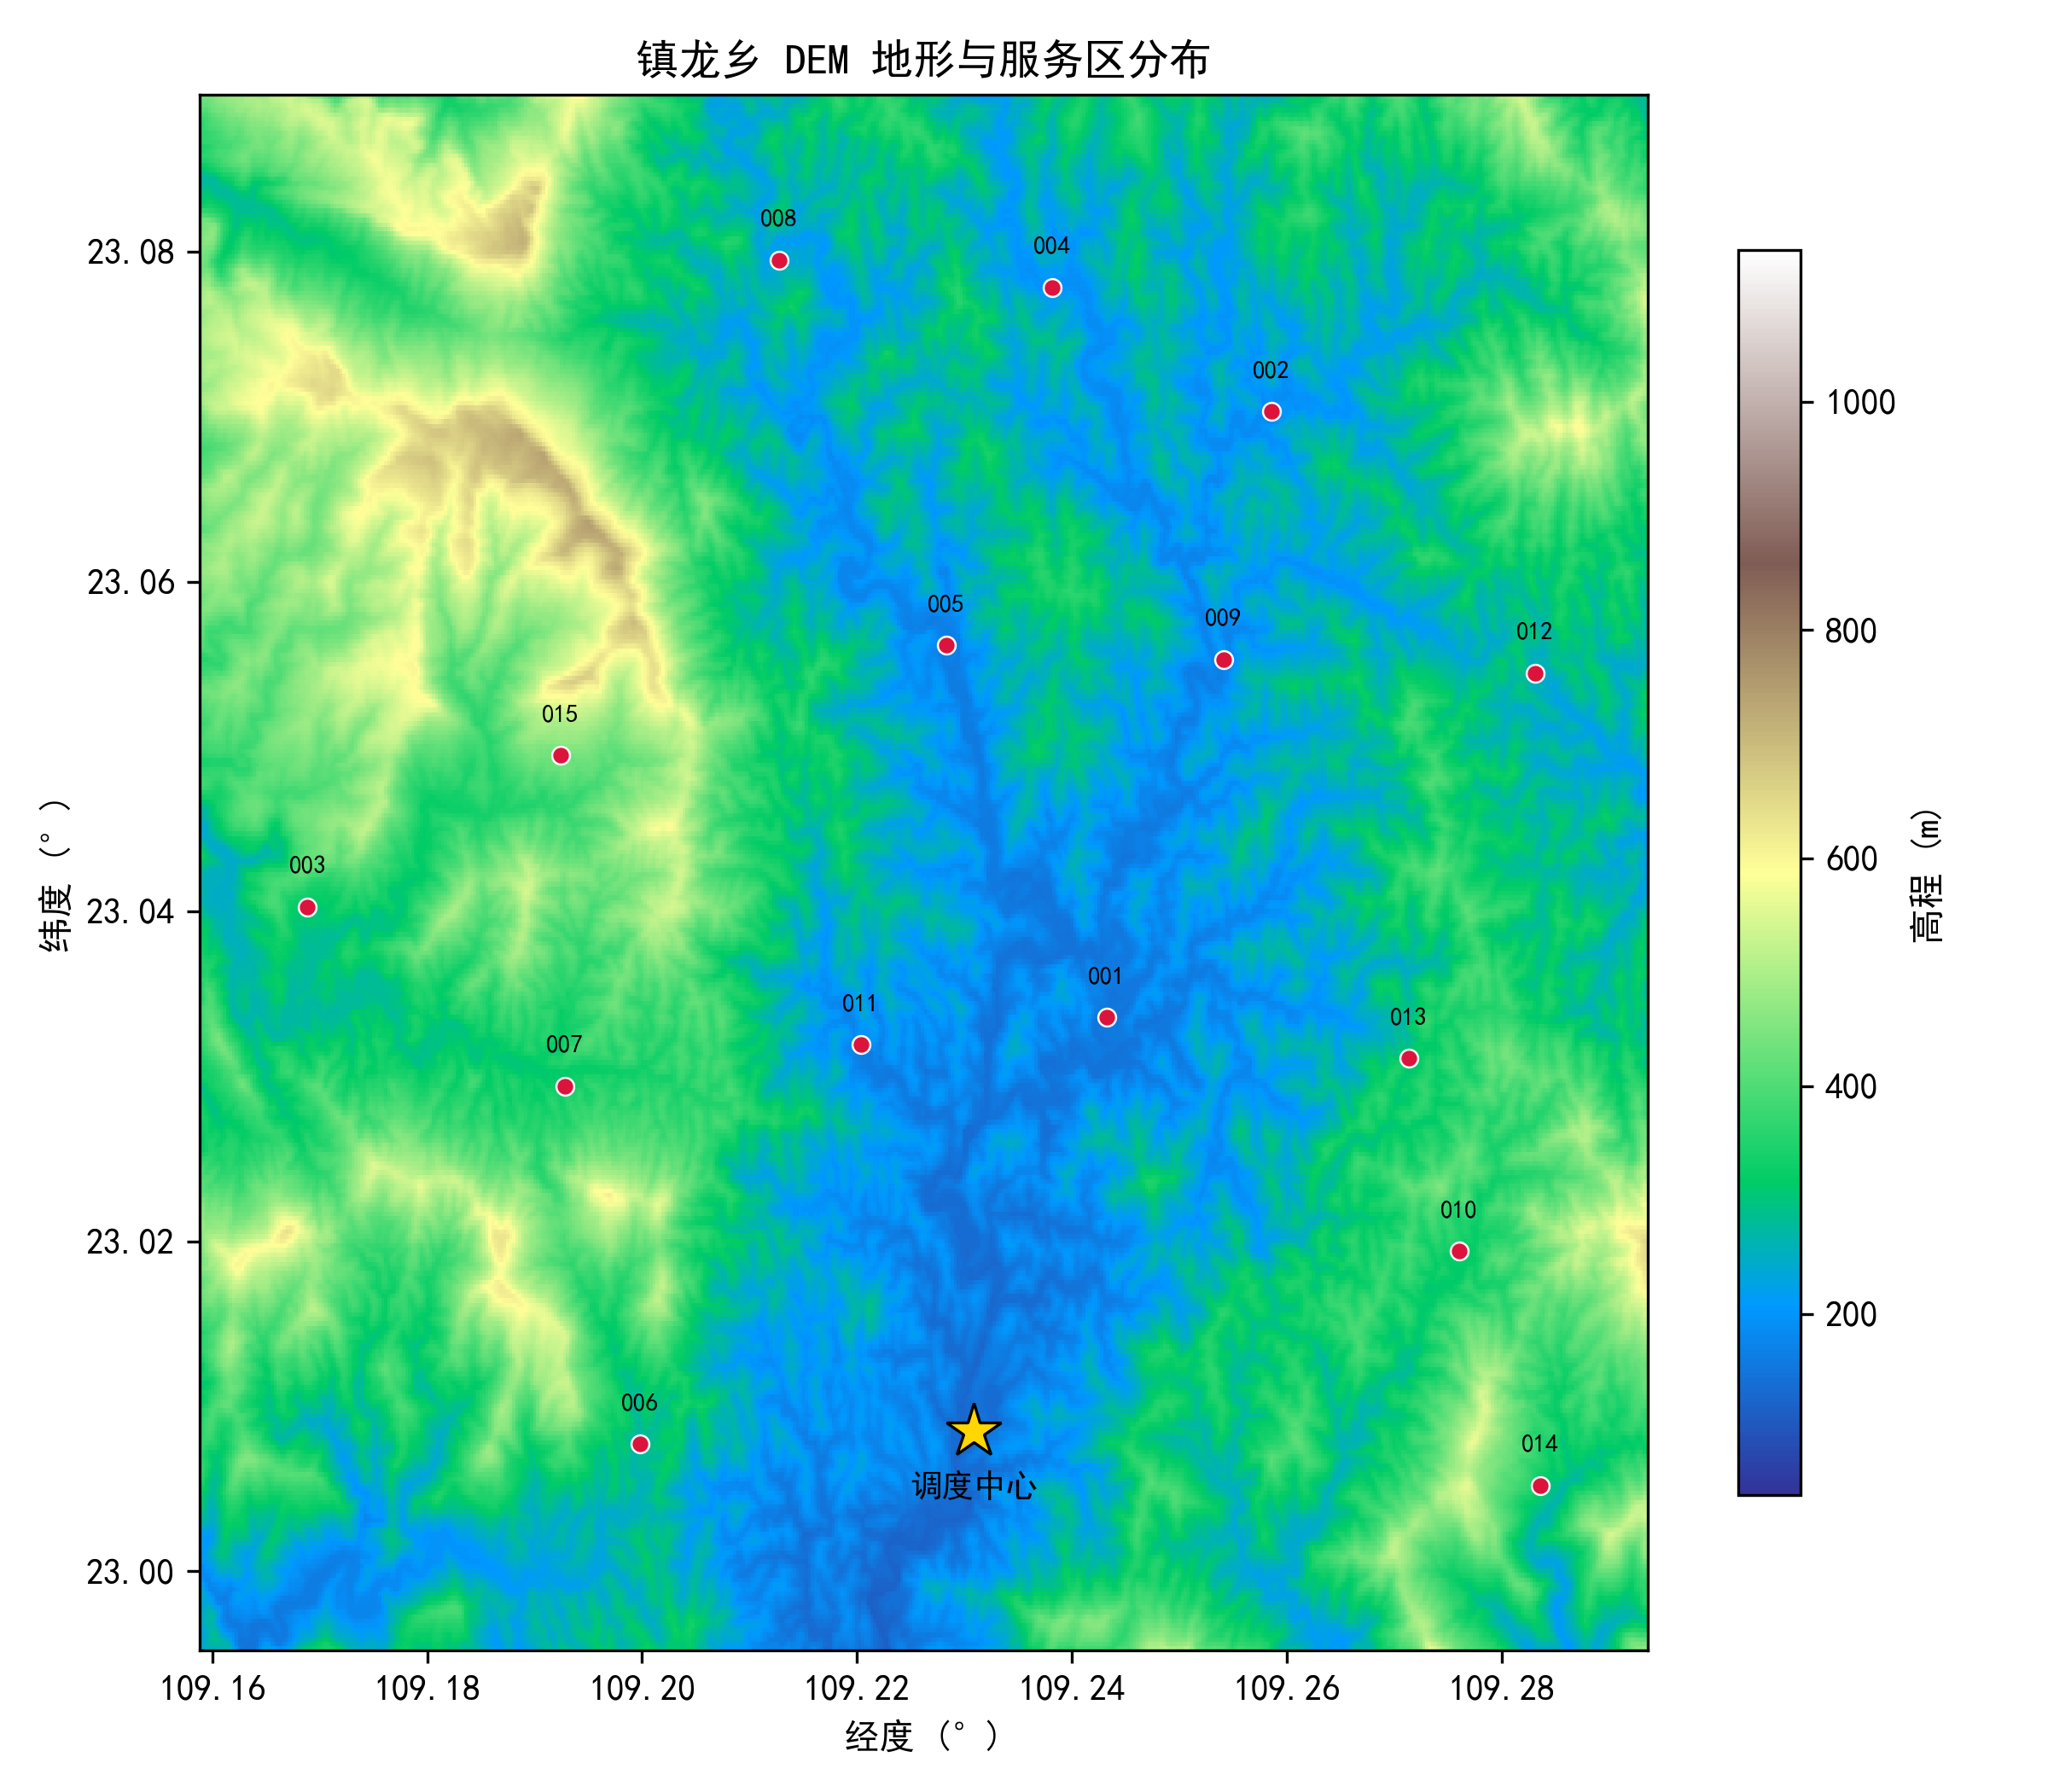
\includegraphics[width=0.82\textwidth]{figures/fig_dem_map.png}
	\caption{镇龙乡 DEM 地形与调度节点分布}
	\label{fig:dem-map}
\end{figure}

图~\ref{fig:dem-map}的地形分布直接决定了后文的三条建模口径。其一，\textbf{调度中心与多数服务区并不在同一个高度带上}：色标跨度约 $200\sim1000$\,m，中部有一条南北向的低海拔谷地，O01 正落在谷底，而 S002、S004、S008、S012 等点位于谷地两侧的较高处——故「同一段航程的两端高差」不能忽略，巡航海拔必须按航段沿线实际经过的地形抬升，而不是取两端点的较大值。其二，\textbf{高差是连续起伏而非台阶}：谷地与西侧、东北侧的高脊之间没有平坦过渡，同一航段会在数公里内跨越数百米的高差，这正是第 4 章把巡航海拔取为「沿线所过 DEM 像元的最高地面高程」而非两点插值的原因。其三，\textbf{谷地对两侧构成天然遮挡}：O01 处在低处，而服务区散布在谷地两侧与更远处，两端点之间的视线很容易被中途的脊线切断——这解释了为什么直连通信并非处处可用，也说明中继需求是地形本身带来的，而不是参数设置偏严所致。

\subsection{问题重述}

\noindent \textbf{问题 1（单点往返运输能力与货箱组批方案）：}在不考虑实体无人机和共享电池调度的前提下，研究单服务区直接往返（O01$\to$S$_i\to$O01）条件下的运输能力与货箱组批。要求计算三种机型在不同服务区的最大安全载荷；在货箱不可拆分且满足载质量、装载体积和返航安全能量余量的条件下确定各服务区货箱组批方案；综合考虑架次数、总能耗和累计作业时间对组批方案进行优化并说明指标权衡；并讨论返航安全余量变化对最大安全载荷和组批结果的影响。

\noindent \textbf{问题 2（异构无人机多点多架次运输调度）：}在不考虑通信保障的情况下，研究异构运输无人机的多点多架次调度。每个运输架次可访问一个或多个服务区并返回 O01，在货箱不可拆、载质量与体积、返航安全余量、无人机与共享电池数量、充电周转及物资时限等约束下，联合确定货箱组批、服务区访问顺序、机型、执行无人机、共享电池及各架次开始时刻，并优化配送及时性、任务完成时间、能耗和架次数。

\noindent \textbf{问题 3（通信约束下的运输与中继联合调度）：}在考虑通信保障的情况下，研究运输无人机与中继无人机的联合调度。运输无人机全程需保持连续通信，直连地面网关不可用时由空中中继无人机保障。要求联合确定运输与中继的组批、时序、机型及中继悬停位置、飞行海拔、服务时段和能源组件分配。

\noindent \textbf{问题 4（救援任务分区与资源配置优化）：}以问题三的联合调度方案为基础，将 15 个服务区划分为 2 个和 3 个任务组（保持已确定的组批、访问顺序、运输与中继安排及通信保障关系不变），分别核算各任务组独立执行所需的各类资源数量，并从资源规模、冗余、组间工作量均衡及与库存的缺口等方面比较两种分区方式。
